\documentclass{article}

\usepackage{ctex}
\usepackage{array}
\usepackage{tabularx}
\usepackage{booktabs}
\usepackage{multirow}
\usepackage{makecell}
\usepackage{graphicx}
\usepackage{amsmath}
\usepackage{lmodern}
\usepackage{amssymb}
\usepackage{amsthm}
\usepackage{listings}
\usepackage{xcolor}
\usepackage{caption}

\captionsetup{ labelformat=empty}

\lstset{
 columns=fixed,       
 numbers=left,                                        % 在左侧显示行号
 numberstyle=\tiny\color{gray},                       % 设定行号格式
 frame=none,                                          % 不显示背景边框
 backgroundcolor=\color[RGB]{245,245,244},            % 设定背景颜色
 keywordstyle=\color[RGB]{40,40,255},                 % 设定关键字颜色
 numberstyle=\footnotesize\color{darkgray},           
 commentstyle=\it\color[RGB]{0,96,96},                % 设置代码注释的格式
 stringstyle=\rmfamily\slshape\color[RGB]{128,0,0},   % 设置字符串格式
 showstringspaces=false,                              % 不显示字符串中的空格
 breaklines=true,                                     % 对过长的代码自动换行
 language=matlab,                                     % 设置语言
}


\begin{document}
\graphicspath{{F:/School/大二下/信号与系统/project/project 1/asset}}
\title{Signal and System Project 1}
\author{HeXiang Huang}
\date{\today}
\maketitle

\tableofcontents

\newpage

\section{Problem 1}
\subsection{Making Continuous-Time Pole-Zero Diagrams}
\subsubsection*{(a)}
use the following code to make the pole-zero diagram of the system
\begin{lstlisting}
%% Example
b = [1 -1];
a = [1 3 2];
zs = roots(b);
ps = roots(a);
figure(1);
subplot(2,2,1)
plot(real(zs),imag(zs),'o');
hold on;
plot(real(ps),imag(ps),'x');
title('Example')
grid;
axis([-3 3 -3 3])

%% Exercise a
% Exercise a1
a = [1 5];
b = [1 2 3];
aroot = roots(a);
broot = roots(b);
subplot(2,2,2)
plot(real(aroot),imag(aroot),'o');
hold on;
plot(real(broot),imag(broot),'x');
title('$H(s)=\frac{s+5}{s^2+2s+3}$','Interpreter','latex')
grid;
axis([-6 2 -2 2])

% Exercise a2
a = [2 5 12];
b = [1 2 10];
aroot = roots(a);
broot = roots(b);
subplot(2,2,3)
plot(real(aroot),imag(aroot),'o');
hold on;
plot(real(broot),imag(broot),'x');
title('$H(s)=\frac{2s^2+5s+12}{s^2+2s+10}$','Interpreter','latex')
grid;
axis([-2 0 -4 4])

% Exercise a3
a = [2 5 12];
b = [1 4 14 20];
aroot = roots(a);
broot = roots(b);
subplot(2,2,4)
plot(real(aroot),imag(aroot),'o');
hold on;
plot(real(broot),imag(broot),'x');
title('$H(s)=\frac{2s^2+5s+12}{(s^2+2s+10)(s+2)}$','Interpreter','latex')
grid;
axis([-3 0 -4 4])
\end{lstlisting}
Then we can get the following pole-zero diagrams
\begin{figure}[h]
    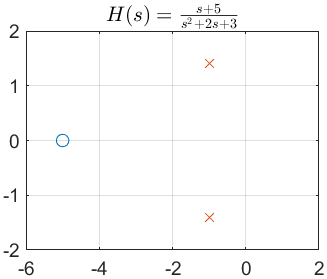
\includegraphics[width = 0.3\textwidth]{1.1.1.2.png}
    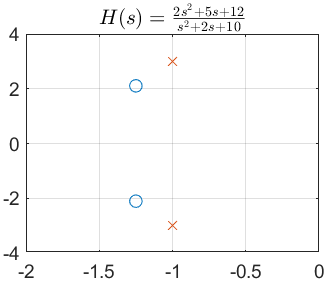
\includegraphics[width = 0.3\textwidth]{1.1.1.3.png}
    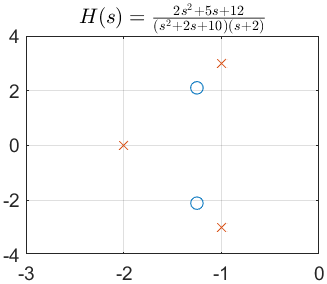
\includegraphics[width = 0.3\textwidth]{1.1.1.4.png}
\end{figure}

\subsubsection*{(b)}
A system is stable when the ROC includes the imaginary axis. 

The poles of $H(s)=\frac{s+5}{s^2+2s+3}$are $s = -1 \pm j\sqrt{2}$,
the system is stable so that the ROC is $Re(s) > -1$

The poles of $H(s) = \frac{2s^2+5s+12}{s^2+2s+10}$are $s = -1 \pm j\sqrt{3}$,
the system is stable so that the ROC is $Re(s) > -1$

The poles of $H(s)=\frac{2s^2+5s+12}{(s^2+2s+10)(s+2)}$are $s = -1 \pm j\sqrt{3}$and $s = -2$,
the system is stable so that the ROC is $Re(s) > -1$

\subsubsection*{(c)}
Do the Laplace transform of the following equations
\begin{center}
    \begin{math}
        \centering
        \frac{dy(t)}{dt} - 3y(t) = \frac{d^2x(t)}{dt^2} + 2\frac{dx(t)}{dt} + x(t)
    \end{math}
\end{center}
we can get
\begin{center}
    \begin{math}
        sY(s) - 3Y(s) = s^2X(s) + 2sX(s) + X(s)
    \end{math}
\end{center}
so that
\begin{center}
    \begin{math}
        H(s) = \frac{Y(s)}{X(s)} = \frac{s^2+2s+1}{s-3}
    \end{math}
\end{center}

The poles of $H(s) = \frac{s^2+2s+1}{s-3}$ are $s = 3$,and the zeros are $s = -1 \pm \sqrt{2}$\\

we can draw the following pole-zero diagrams
\begin{center}
    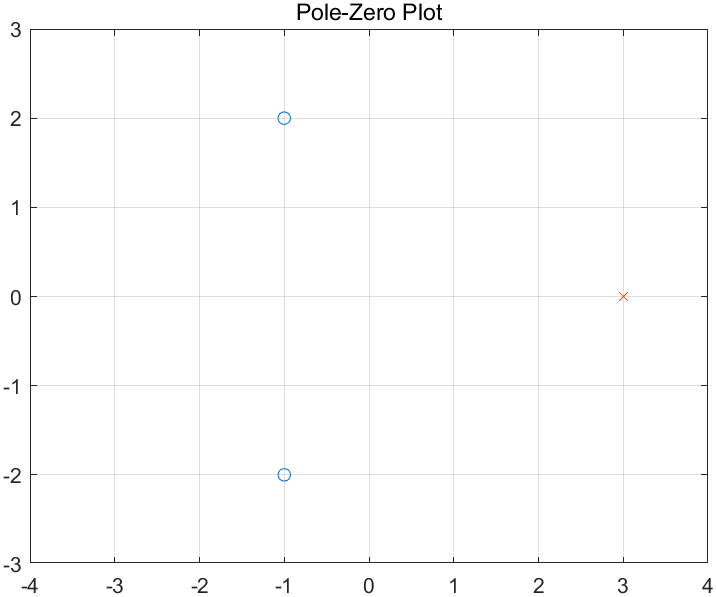
\includegraphics[width = 0.7\textwidth]{1.1.3.png}
\end{center}

\subsubsection*{(d)}
In the function "pzplot",it use the function "roots" to find the poles and zeros of the system, and then plot the poles and zeros on the complex plane.
for every pole, if the pole is on the left side of the given point,the ROC should contain the right side of the pole, and if the pole is on the right side of the given point, the ROC should contain the left side of the pole.\\
\subsection{Making Discrete-Time Pole-Zero Diagrams}

\subsubsection*{Note}

In the M-file "dpzplot.m", it use the outdated function \bf{"clg"},in order to inform that the function works well,we use the function \bf{"clf"} instead of \bf{"clg"}.\\
\begin{lstlisting}
    %clg;
    clf;
\end{lstlisting}

\subsubsection*{(a)}
use the following easy code to make the pole-zero diagram of the system
\begin{lstlisting}
b = [1 -1 0];  % 分子系数
a = [1 3 2];   % 分母系数
dpzplot(b, a); % 绘制零极点图
\end{lstlisting}
Then we can get the following pole-zero diagrams
\begin{center}
    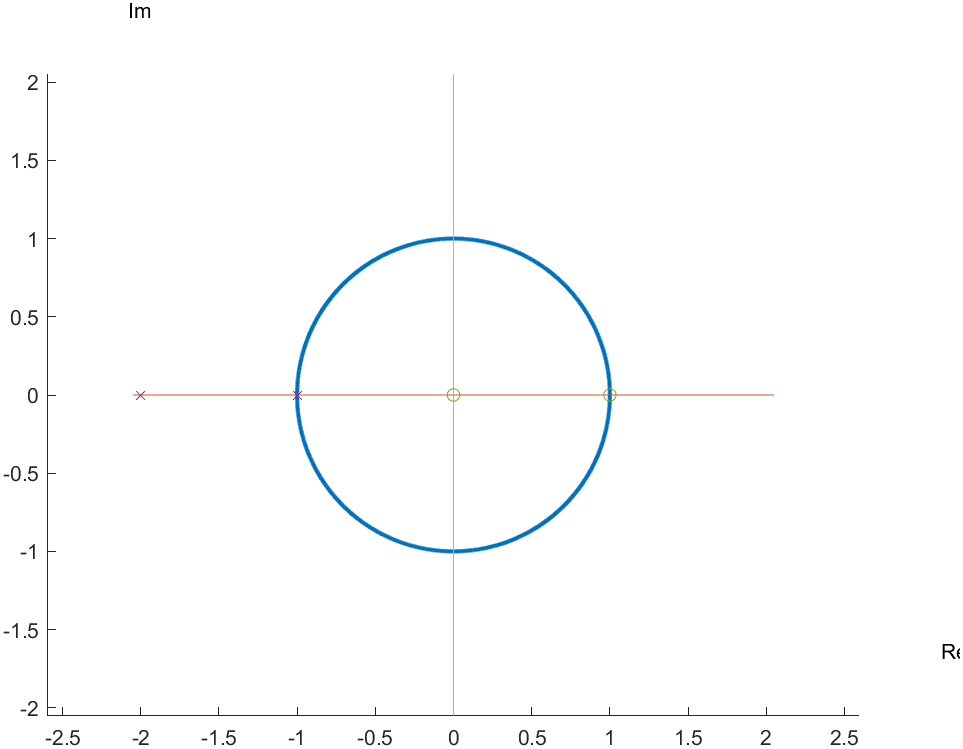
\includegraphics[width = 0.7\textwidth]{1.2.1.png}
\end{center}

\subsubsection*{(b)}

Do the Z-transform of the following equations
\begin{center}
    \begin{math}
        \centering
        y[n] +y[n-1] + 0.5y[n-2] = x[n]
    \end{math}
\end{center}
we can get
\begin{center}
    \begin{math}
        Y(z) + Y(z)z^{-1} + 0.5Y(z)z^{-2} = X(z)
    \end{math}
\end{center}
so that
\begin{center}
    \begin{math}
        H(z) = \frac{Y(z)}{X(z)} = \frac{1}{1+z^{-1}+0.5z^{-2}} = \frac{z^2}{z^2+z+0.5}
    \end{math}
\end{center}
use the following code we can get the following pole-zero diagrams
\begin{lstlisting}
b = [1 0 0];      % 分子系数
a = [1 1 0.5];    % 分母系数
dpzplot(b, a);    % 绘制零极点图
\end{lstlisting}
\begin{center}
    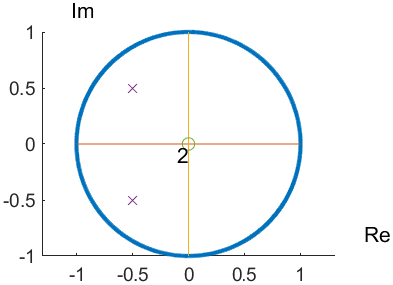
\includegraphics[width = 0.7\textwidth]{1.2.2.png}
\end{center}

\subsubsection*{(c)}
Do the Z-transform of the following equations
\begin{center}
    \begin{math}
        \centering
        y[n] - 1.25y[n-1] +0.75y[n-2]-0.125y[n-3] = x[n] +0.5x[n-1]
    \end{math}
\end{center}
we can get
\begin{center}
    \begin{math}
        Y(z) - 1.25Y(z)z^{-1} + 0.75Y(z)z^{-2} - 0.125Y(z)z^{-3} = X(z) + 0.5X(z)z^{-1}
    \end{math}
\end{center}
so that
\begin{center}
    \begin{math}
        H(z) = \frac{Y(z)}{X(z)} = \frac{1+0.5z^{-1}}{1-1.25z^{-1}+0.75z^{-2}-0.125z^{-3}} = \frac{z^3+0.5z^2}{z^3-1.25z^2+0.75z-0.125}
    \end{math}
\end{center}
use the following code we can get the following pole-zero diagrams
\begin{lstlisting}
b = [1 0.5 0 0];      % 分子系数
a = [1 -1.25 0.75 -0.125];    % 分母系数
dpzplot(b, a);    % 绘制零极点图
\end{lstlisting}
\begin{center}
    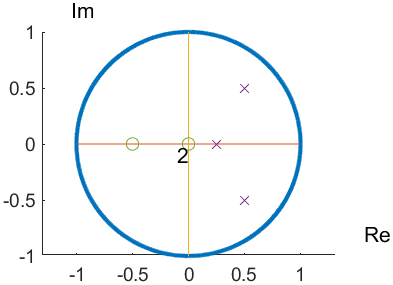
\includegraphics[width = 0.7\textwidth]{1.2.3.png}
\end{center}

\newpage
\section{Problem 2}
\subsection{Smiley}
\subsubsection*{(a)}
\begin{center}
    \begin{math}
        y[n] = (p*x)[n] = \sum_{k=-\infty}^{\infty}x[k]p[n-k]
    \end{math}
\end{center}
In order to make y[n] maximized when n=2,we need to make $x[k]p[2-k] = 1$for $k = 1,2,3$
and $x[k]p[2-k] = 1$for other k.

So we can get the following p[n]
\begin{center}
    \begin{align*}
        p[-1] &= 1\\
        p[0] &= -1\\
        p[1] &= -1\\
        p[n] &= 0 , n \not =0,\pm 1
    \end{align*}
\end{center}

\subsubsection*{(b)}
Now let we turn to finding nose.\par
Using the initial value of white and black pixels,we can 
notice that the white pixels contribute positive to the answer if they match 
but the black pixels contribute zero to the answer whether or not match.
So we firstly substract 127.5 from the pixel value so that 
black pixels and white pixels both contribute positively to the answer if they match 
and contribute negative when they don't match.One step further,
we can normalize$\pm 127.5$to $\pm 1$\par

Consider above process,the feature of nose is the following matrix
\begin{center}
    \begin{math}
        \begin{bmatrix}
            -1 & -1 & -1 & -1 & -1\\
            -1 & 1 & -1 & 1 & -1\\
            -1 & -1 & 1 & -1 & -1\\
            -1 & -1 & -1 & -1 & -1\\
            -1 & 1 & 1 & 1 & -1\\
            -1 & -1 & -1 & -1 & -1
        \end{bmatrix}
    \end{math}
\end{center}
Consider the two-dimensional convolution and make y[n,m] maximized when [n,m]
matches the row and column of the nose,we can get the following p[n,m]
\begin{center}
    \begin{math}
        \begin{bmatrix}
            -1 & -1 & -1 & -1 & -1\\
            -1 & 1 & 1 & 1 & -1\\
            -1 & -1 & -1 & -1 & -1\\
            -1 & -1 & 1 & -1 & -1\\
            -1 & 1 & -1 & 1 & -1\\
            -1 & -1 & -1 & -1 & -1
        \end{bmatrix}
    \end{math}
\end{center}
We can use the following code to get the position of nose
\begin{lstlisting}
clc;
close all;
clear;
%read the image
img = imread("F:\School\大二下\信号与系统\project\project 1\introduction\Files for Problem2\findsmiley.jpg");
[img_row,img_colum] = size(img);
%turn to double type in order to normalize the matrix
img_copy = double(img);
for i = 1:img_row
    for j =1:img_colum
        if(img_copy(i,j)>200)
            img_copy(i,j) = 1;
        else
            img_copy(i,j) = -1;
        end
    end
end
%create the matching matrix
p = [-1 -1 -1 -1 -1;
    -1 1 1 1 -1;
    -1 -1 -1 -1 -1;
    -1 -1 1 -1 -1;
    -1 1 -1 1 -1;
    -1 -1 -1 -1 -1];
sum = 0;
sum_max = 0;
nose_row = 0;
nose_colum = 0;
%do the convolution
for i =3:img_row-3
    for j=3:img_colum-2
        img_matrix = img_copy(i-2:i+3,j-2:j+2);
        for k = -2:3
            for l =-2:2
                sum = sum+img_matrix(3+k,3+l)*p(4-k,3-l);
            end
        end
        if(sum>sum_max)
            nose_row = i;
            nose_colum =j;
            sum_max = sum;
        end
        sum = 0;
    end
end
%show the image
smiley_img = img(nose_row-2:nose_row+3,nose_colum-2:nose_colum+2);
imshow(smiley_img,'InitialMagnification','fit')
\end{lstlisting}
Run the code and we can konw that \bf{the row of nose is 124} and 
\bf{the column of nose is 900} and we can get the following image
\begin{center}
    
\includegraphics[width = 0.7\textwidth]{2.2.png}
\end{center}

\subsubsection*{(c)}
The problem requires us to add noise to the image and 
use the same metheod to find the nose.But I found that 
the noise alreadly exists in the image,so I firstly clean 
the noise and then add noise to the image in order to 
use the function "normrnd".\par
We can get the smiley without noise by the following code
\begin{lstlisting}
clc;
close all;
clear;

%read imag
img = imread("F:\School\大二下\信号与系统\project\project 1\introduction\Files for Problem2\findsmiley.jpg");
[img_row,img_colum] = size(img);
img_copy = img;
% clean the noise
for i = 1:img_row
    for j =1:img_colum
        if(img_copy(i,j)>200)
            img_copy(i,j) = 255;
        else
            img_copy(i,j) = 0;
        end
    end
end
%save imag
imwrite(img_copy,'F:\School\大二下\信号与系统\project\project 1\asset\smiley_without_noise.png')
\end{lstlisting}
Now let us process the image without noise.\par
Because of the noise,we can't normalize$\pm 127.5$to $\pm 1$,
so I just substract 127.5 from the pixel value.\par
Use the similar code(more detail in 2c code segment in "problem2.m") ,
we can get that the row of nose is 124 and
the column of nose is 900 and we can get the following image
\begin{center}
    
\includegraphics[width = 0.7\textwidth]{2.3.png}
\end{center}
We can see that the method works well even if the image has some noise.
\newpage
\section{Problem 3}

\subsection{Use the Sounds in Matlab}
Using the following code, you can get the wave of the sound and play it.
\begin{lstlisting}
clc;
close all;
clear;

% read .wav
[y, Fs] = audioread('snare.wav'); 

% draw the wave
t = (0:length(y)-1)/Fs; 
plot(t, y);
xlabel('Time (s)');
ylabel('Amplitude');

% play the .wav
sound(y, Fs); 
\end{lstlisting}
Some sound is too short to be listened clearly,but 
the sounds that can be listened clearly roughly 
meet my expectation.Now I put the wave of the sound.
\begin{figure}[h]
    \begin{minipage}{0.45\textwidth}
        \centering
        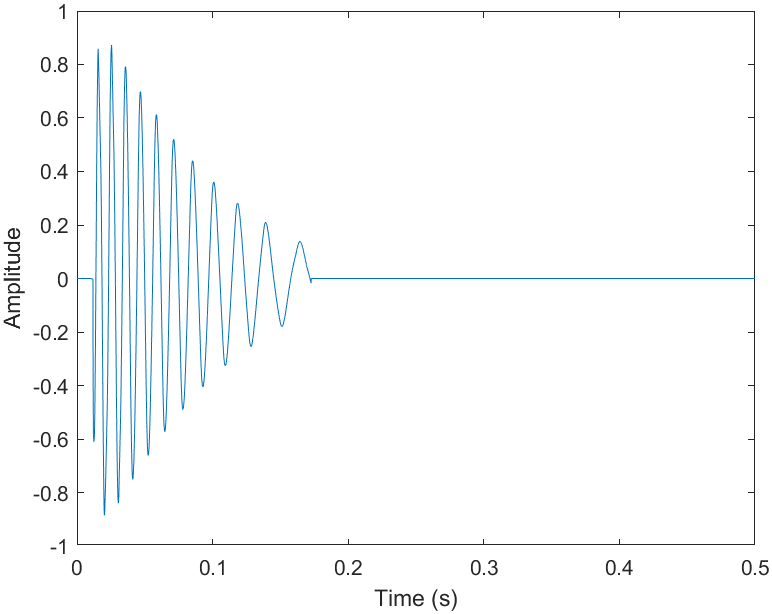
\includegraphics[width=0.8\linewidth]{3.1bassdrum.png}
        \caption{bassdrum}
    \end{minipage}
    \begin{minipage}{0.45\textwidth}
        \centering
        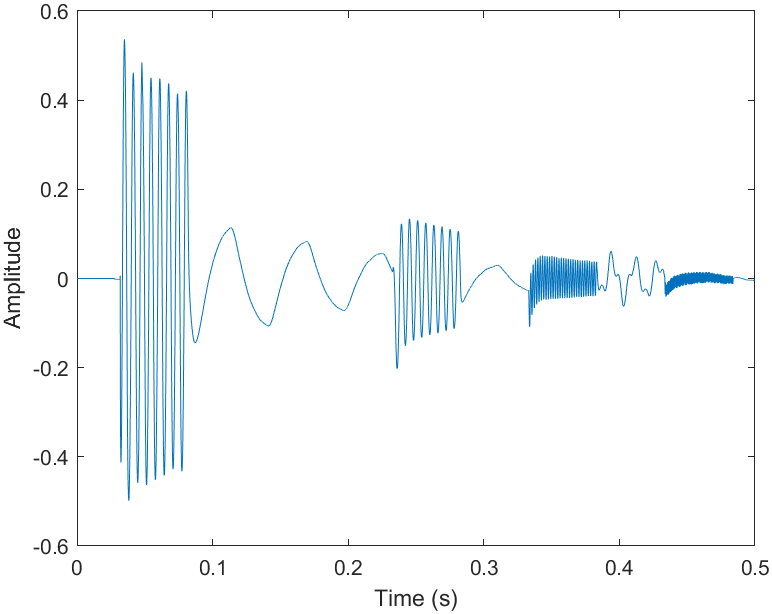
\includegraphics[width=0.8\linewidth]{3.1bleeep.png}
        \caption{bleeep}
    \end{minipage}
    \quad

    \begin{minipage}{0.45\textwidth}
        \centering
        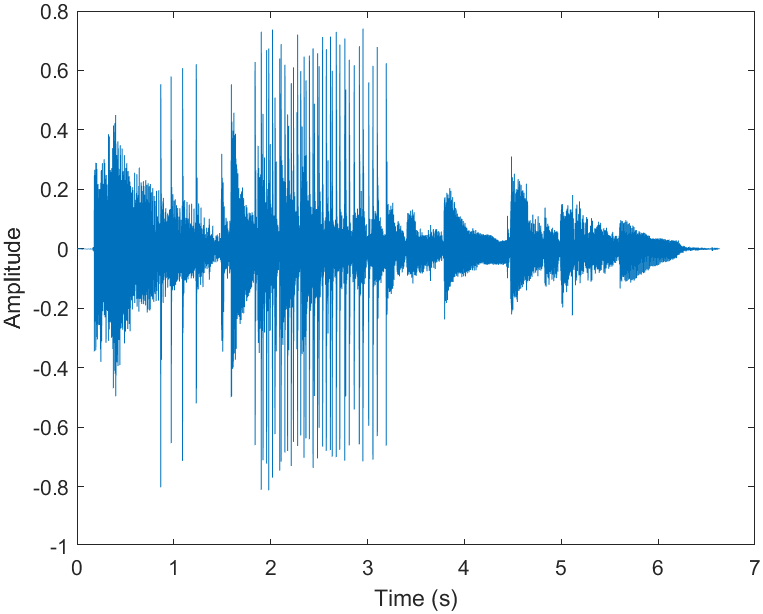
\includegraphics[width=0.8\linewidth]{3.1castanets44m.png}
        \caption{castanets44m}
    \end{minipage}
    \begin{minipage}{0.45\textwidth}
        \centering
        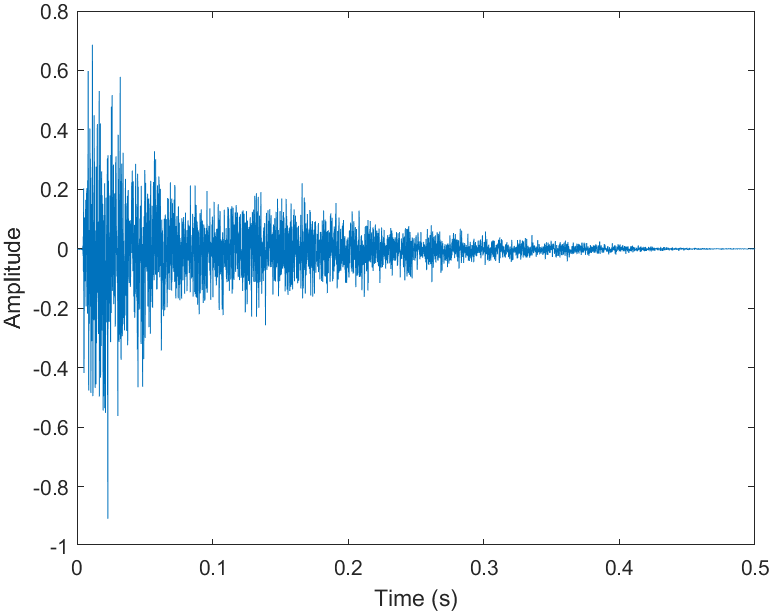
\includegraphics[width=0.8\linewidth]{3.1hatclosed.png}
        \caption{hatclosed}
    \end{minipage}
    \quad

    \begin{minipage}{0.45\textwidth}
        \centering
        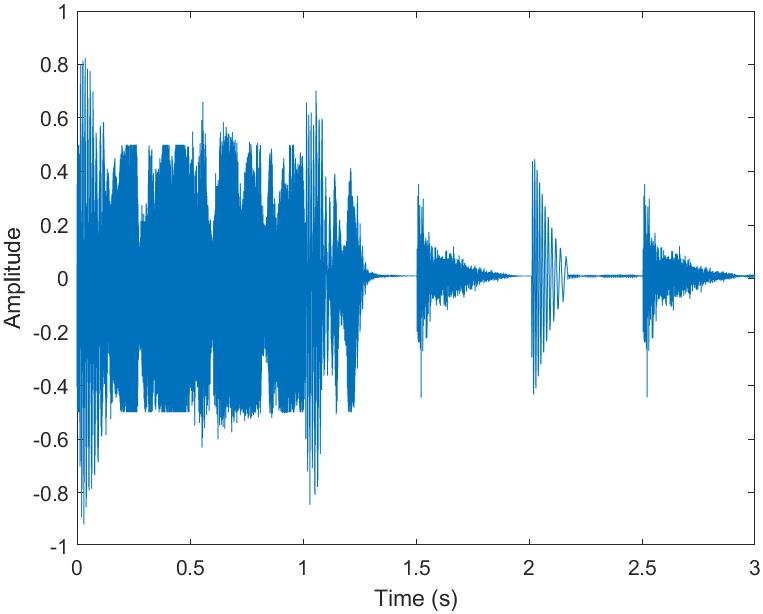
\includegraphics[width=0.8\linewidth]{3.1mixed.png}
        \caption{mixed}
    \end{minipage}
    \begin{minipage}{0.45\textwidth}
        \centering
        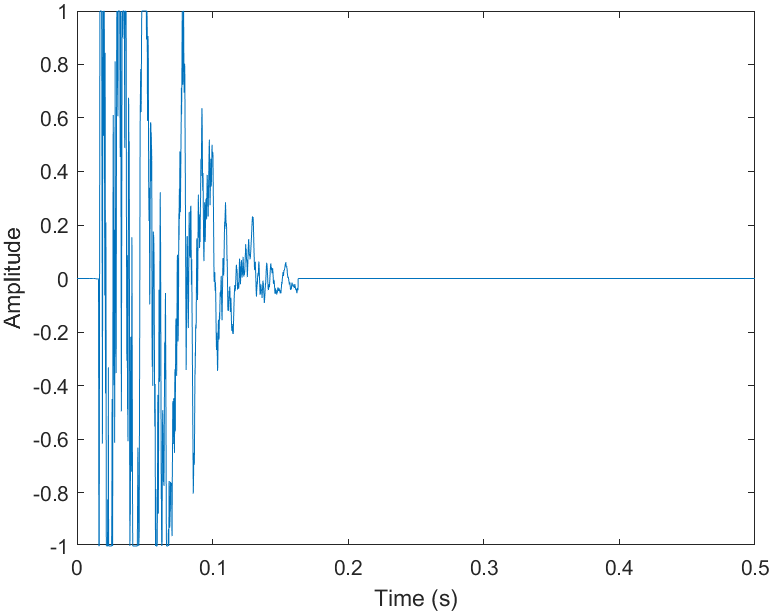
\includegraphics[width=0.8\linewidth]{3.1snare.png}
        \caption{snare}
    \end{minipage}
\end{figure} 

\newpage
\subsubsection*{A.Time-reverse \& Timescale}
The sound vector is a column vector, 
so we can use the function "flipud".\par
In "TimeReverse.m"
\begin{lstlisting}
function sound_rev = TimeReverse(y)
    sound_rev = flipud(y);
end
\end{lstlisting}
In "problem3.m"
\begin{lstlisting}
clc;
close all;
clear;

[y, Fs] = audioread('castanets44m.wav');
y_rev = TimeReverse(y);
% draw the wave
t = (0:length(y)-1)/Fs;

figure(1)
subplot(1,2,1)
plot(t, y);
xlabel('Time (s)');
ylabel('Amplitude');

subplot(1,2,2)
plot(t, y_rev);
xlabel('Time (s)');
ylabel('Amplitude');

% play the sound
sound(y_rev, Fs);
\end{lstlisting} 

\newpage
We can get two compared wave of the sound.
\begin{figure}[h]
    \begin{minipage}{0.45\textwidth}
        \centering
        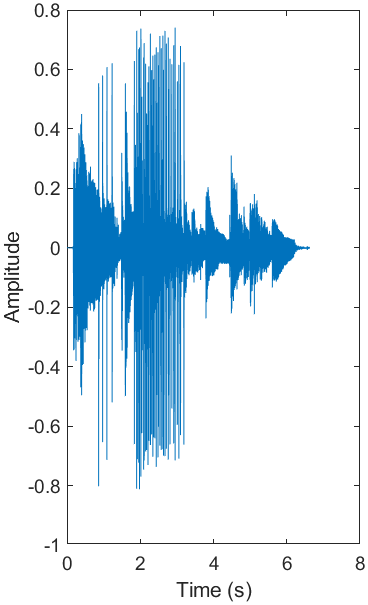
\includegraphics[width=0.8\linewidth]{3.1A2.png}
        \caption{origin wave}
    \end{minipage}
    \begin{minipage}{0.45\textwidth}
        \centering
        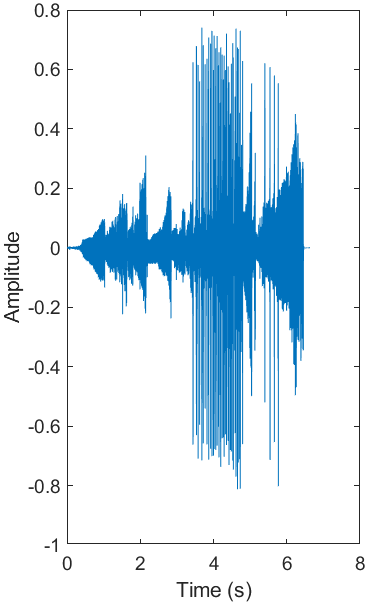
\includegraphics[width=0.8\linewidth]{3.1A1.png}
        \caption{reversed wave}
    \end{minipage}
\end{figure}

\par
When use the function "timescale",the pitch changes with the change of the frequency of the sound.

\subsubsection*{B.Fader}
In "fade.m"
\begin{lstlisting}
% process the level
if(level>1)
    level = 1;
elseif(level<0)
    level = 0;
end

%create the ramp vector
t = linspace(1,level,length(x));
% multiply the audio vector with the ramp vector to fade
y = t .* x;
\end{lstlisting}
Using the function(more detail in "problem3.m"),we can get the following plot.
\begin{figure}[h]
    \begin{minipage}{0.45\textwidth}
        \centering
        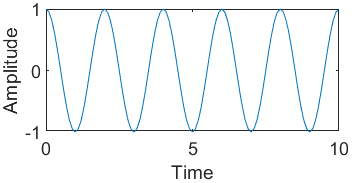
\includegraphics[width=0.8\linewidth]{3.1B1.png}
        \caption{Input y}
    \end{minipage}
    \begin{minipage}{0.45\textwidth}
        \centering
        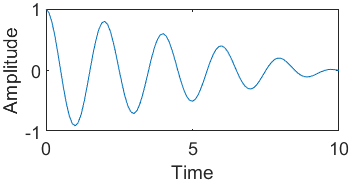
\includegraphics[width=0.8\linewidth]{3.1B2.png}
        \caption{Level = 0 or -2}
    \end{minipage}
    \quad

    \begin{minipage}{0.45\textwidth}
        \centering
        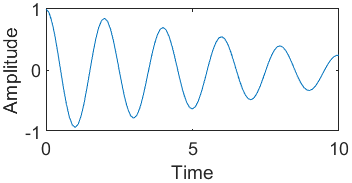
\includegraphics[width=0.8\linewidth]{3.1B3.png}
        \caption{Level = 0.25}
    \end{minipage}
    \begin{minipage}{0.45\textwidth}
        \centering
        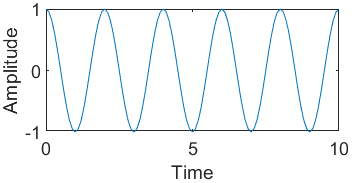
\includegraphics[width=0.8\linewidth]{3.1B1.png}
        \caption{Level = 100}
    \end{minipage}
\end{figure}

\subsubsection*{C.Repeater}
In "repeat.m"
\begin{lstlisting}
function out = repeat(sound,N)

%process N
if(N<0)
    N = 0;
end
% turn N to integer
N = fix(N);

% repeat the sound
if(N==0)
    out = sound;
else
    out = sound;
    for i=1:N
        out = [out;sound];
    end
end
\end{lstlisting}
Using the function(more detail in "problem3.m"),we can get the following plot.
\begin{figure}[h]
    \begin{minipage}{0.45\textwidth}
        \centering
        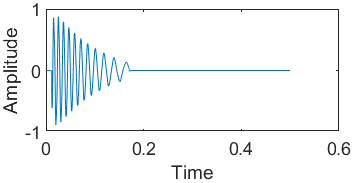
\includegraphics[width=0.8\linewidth]{3.1C1.png}
        \caption{Input sound}
    \end{minipage}
    \begin{minipage}{0.45\textwidth}
        \centering
        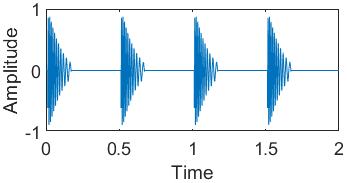
\includegraphics[width=0.8\linewidth]{3.1C2.png}
        \caption{N = 3}
    \end{minipage}
    \quad

    \begin{minipage}{0.45\textwidth}
        \centering
        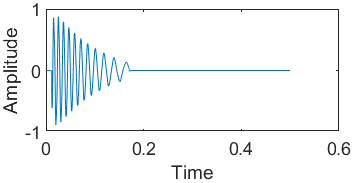
\includegraphics[width=0.8\linewidth]{3.1C1.png}
        \caption{N = 0}
    \end{minipage}
    \begin{minipage}{0.45\textwidth}
        \centering
        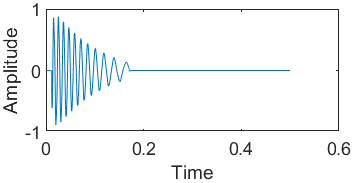
\includegraphics[width=0.8\linewidth]{3.1C1.png}
        \caption{N = -1}
    \end{minipage}
\end{figure}

\subsubsection*{D.Delay}
In "delay.m"
\begin{lstlisting}
function out =delay(sound,delay,Fs)

if(delay>0)
    zero_length = delay*Fs;
    zero_sound = zeros(zero_length,1);
    out = [zero_sound;sound];
elseif(delay == 0)
    out = sound;
else
    advance_length = -delay*Fs;
    if(advance_length<length(sound))
        out = sound((advance_length+1):length(sound),:);
    else
        out = 0;
    end
end
\end{lstlisting}
Use the function(more detail in "problem3.m"),we can get the following plot.\par
\begin{figure}[h]
    \begin{minipage}{0.45\textwidth}
        \centering
        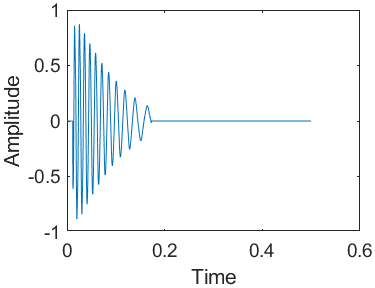
\includegraphics[width=0.8\linewidth]{3.1D1.png}
        \caption{Input sound}
    \end{minipage}
    \begin{minipage}{0.45\textwidth}
        \centering
        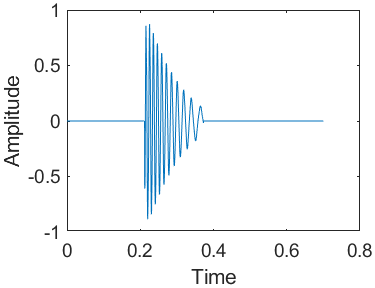
\includegraphics[width=0.8\linewidth]{3.1D2.png}
        \caption{delay = 0.2}
    \end{minipage}
    \quad

    \begin{minipage}{0.45\textwidth}
        \centering
        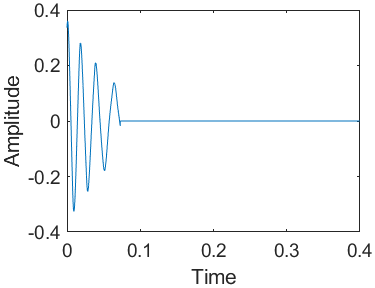
\includegraphics[width=0.8\linewidth]{3.1D3.png}
        \caption{delay = -0.1}
    \end{minipage}
    \begin{minipage}{0.45\textwidth}
        \centering
        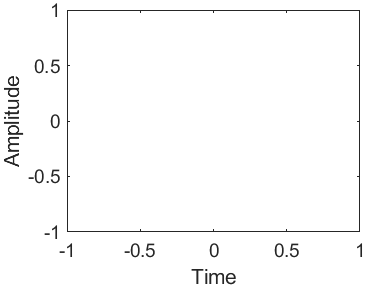
\includegraphics[width=0.8\linewidth]{3.1D4.png}
        \caption{delay = -1}
    \end{minipage}
\end{figure}
When I delay by a negative number, I put the sound advance.

\subsubsection*{E.Mixer}
In order to provide more options for users,
I offer gain1 for sound1 and gain2 for sound2.
In the function I want to mix two sounds with 
both feature of sounds saved.So I firstly process 
gain1 and gain2 and in result gain1 plus gain2 equals to 1. 
In the end of the funtion, I try to amplify the sound 
so that the sound can be listened clearly.\par
In "mixer.m"\par
\begin{lstlisting} 
function out = mix(sound1, sound2,gain1, gain2)

sound_copy1 = sound1;
sound_copy2 = sound2;

gainf1 = gain1/(gain1+gain2);
gainf2 = gain2/(gain1+gain2);

length1 = length(sound1);
length2 = length(sound2);
maxlength = max(length1,length2);
if(length1<maxlength)
    zerolength = maxlength-length1;
    zerosound = zeros(zerolength,1);
    sound_copy1 = [sound_copy1;zerosound];
end

if(length2<maxlength)
    zerolength = maxlength-length2;
    zerosound = zeros(zerolength,1);
    sound_copy2 = [sound_copy2;zerosound];
end

out = sound_copy1.*gainf1+sound_copy2.*gainf2;
maxAmp = max(abs(out));
out = out.*(1/maxAmp);
\end{lstlisting}
\newpage
Using the function(more detail in "problem3.m")with gain1 =3 and gain2 = 2,
we can get the following plot.\par
\begin{figure}[h]
    \begin{minipage}{1.0\textwidth}
        \centering
        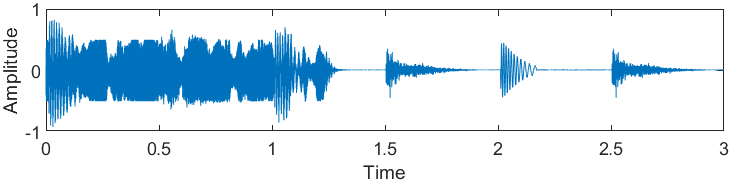
\includegraphics[width=0.8\linewidth]{3.1E1.png}
        \caption{sound1}
    \end{minipage}

    \quad

    \begin{minipage}{1.0\textwidth}
        \centering
        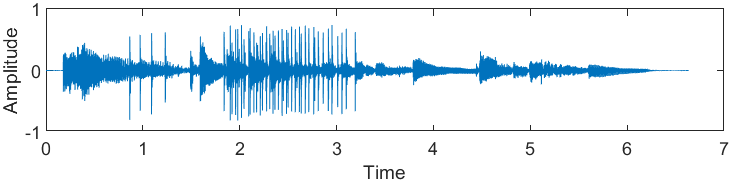
\includegraphics[width=0.8\linewidth]{3.1E2.png}
        \caption{sound2}
    \end{minipage}

    \quad

    \begin{minipage}{1.0\textwidth}
        \centering
        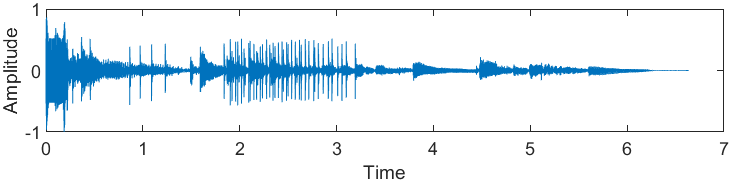
\includegraphics[width=0.8\linewidth]{3.1E3.png}
        \caption{mix sound}
    \end{minipage}
\end{figure}

\subsection{Make Your Own Music}

The function "note" is used to generate a note with particular frequency and duration.
The function "generate\_melody" is used to generate a melody with a sequence of notes.
The "HexiangHuang.m" is the main code.
You can find more detail in the fold "src".\par
The wav file is saved in the fold "asset".\par
\end{document}